\documentclass[1p]{elsarticle_modified}
%\bibliographystyle{elsarticle-num}

%\usepackage[colorlinks]{hyperref}
%\usepackage{abbrmath_seonhwa} %\Abb, \Ascr, \Acal ,\Abf, \Afrak
\usepackage{amsfonts}
\usepackage{amssymb}
\usepackage{amsmath}
\usepackage{amsthm}
\usepackage{scalefnt}
\usepackage{amsbsy}
\usepackage{kotex}
\usepackage{caption}
\usepackage{subfig}
\usepackage{color}
\usepackage{graphicx}
\usepackage{xcolor} %% white, black, red, green, blue, cyan, magenta, yellow
\usepackage{float}
\usepackage{setspace}
\usepackage{hyperref}

\usepackage{tikz}
\usetikzlibrary{arrows}

\usepackage{multirow}
\usepackage{array} % fixed length table
\usepackage{hhline}

%%%%%%%%%%%%%%%%%%%%%
\makeatletter
\renewcommand*\env@matrix[1][\arraystretch]{%
	\edef\arraystretch{#1}%
	\hskip -\arraycolsep
	\let\@ifnextchar\new@ifnextchar
	\array{*\c@MaxMatrixCols c}}
\makeatother %https://tex.stackexchange.com/questions/14071/how-can-i-increase-the-line-spacing-in-a-matrix
%%%%%%%%%%%%%%%

\usepackage[normalem]{ulem}

\newcommand{\msout}[1]{\ifmmode\text{\sout{\ensuremath{#1}}}\else\sout{#1}\fi}
%SOURCE: \msout is \stkout macro in https://tex.stackexchange.com/questions/20609/strikeout-in-math-mode

\newcommand{\cancel}[1]{
	\ifmmode
	{\color{red}\msout{#1}}
	\else
	{\color{red}\sout{#1}}
	\fi
}

\newcommand{\add}[1]{
	{\color{blue}\uwave{#1}}
}

\newcommand{\replace}[2]{
	\ifmmode
	{\color{red}\msout{#1}}{\color{blue}\uwave{#2}}
	\else
	{\color{red}\sout{#1}}{\color{blue}\uwave{#2}}
	\fi
}

\newcommand{\Sol}{\mathcal{S}} %segment
\newcommand{\D}{D} %diagram
\newcommand{\A}{\mathcal{A}} %arc


%%%%%%%%%%%%%%%%%%%%%%%%%%%%%5 test

\def\sl{\operatorname{\textup{SL}}(2,\Cbb)}
\def\psl{\operatorname{\textup{PSL}}(2,\Cbb)}
\def\quan{\mkern 1mu \triangleright \mkern 1mu}

\theoremstyle{definition}
\newtheorem{thm}{Theorem}[section]
\newtheorem{prop}[thm]{Proposition}
\newtheorem{lem}[thm]{Lemma}
\newtheorem{ques}[thm]{Question}
\newtheorem{cor}[thm]{Corollary}
\newtheorem{defn}[thm]{Definition}
\newtheorem{exam}[thm]{Example}
\newtheorem{rmk}[thm]{Remark}
\newtheorem{alg}[thm]{Algorithm}

\newcommand{\I}{\sqrt{-1}}
\begin{document}

%\begin{frontmatter}
%
%\title{Boundary parabolic representations of knots up to 8 crossings}
%
%%% Group authors per affiliation:
%\author{Yunhi Cho} 
%\address{Department of Mathematics, University of Seoul, Seoul, Korea}
%\ead{yhcho@uos.ac.kr}
%
%
%\author{Seonhwa Kim} %\fnref{s_kim}}
%\address{Center for Geometry and Physics, Institute for Basic Science, Pohang, 37673, Korea}
%\ead{ryeona17@ibs.re.kr}
%
%\author{Hyuk Kim}
%\address{Department of Mathematical Sciences, Seoul National University, Seoul 08826, Korea}
%\ead{hyukkim@snu.ac.kr}
%
%\author{Seokbeom Yoon}
%\address{Department of Mathematical Sciences, Seoul National University, Seoul, 08826,  Korea}
%\ead{sbyoon15@snu.ac.kr}
%
%\begin{abstract}
%We find all boundary parabolic representation of knots up to 8 crossings.
%
%\end{abstract}
%\begin{keyword}
%    \MSC[2010] 57M25 
%\end{keyword}
%
%\end{frontmatter}

%\linenumbers
%\tableofcontents
%
\newcommand\colored[1]{\textcolor{white}{\rule[-0.35ex]{0.8em}{1.4ex}}\kern-0.8em\color{red} #1}%
%\newcommand\colored[1]{\textcolor{white}{ #1}\kern-2.17ex	\textcolor{white}{ #1}\kern-1.81ex	\textcolor{white}{ #1}\kern-2.15ex\color{red}#1	}

{\Large $\underline{12a_{0783}~(K12a_{0783})}$}

\setlength{\tabcolsep}{10pt}
\renewcommand{\arraystretch}{1.6}
\vspace{1cm}\begin{tabular}{m{100pt}>{\centering\arraybackslash}m{274pt}}
\multirow{5}{120pt}{
	\centering
	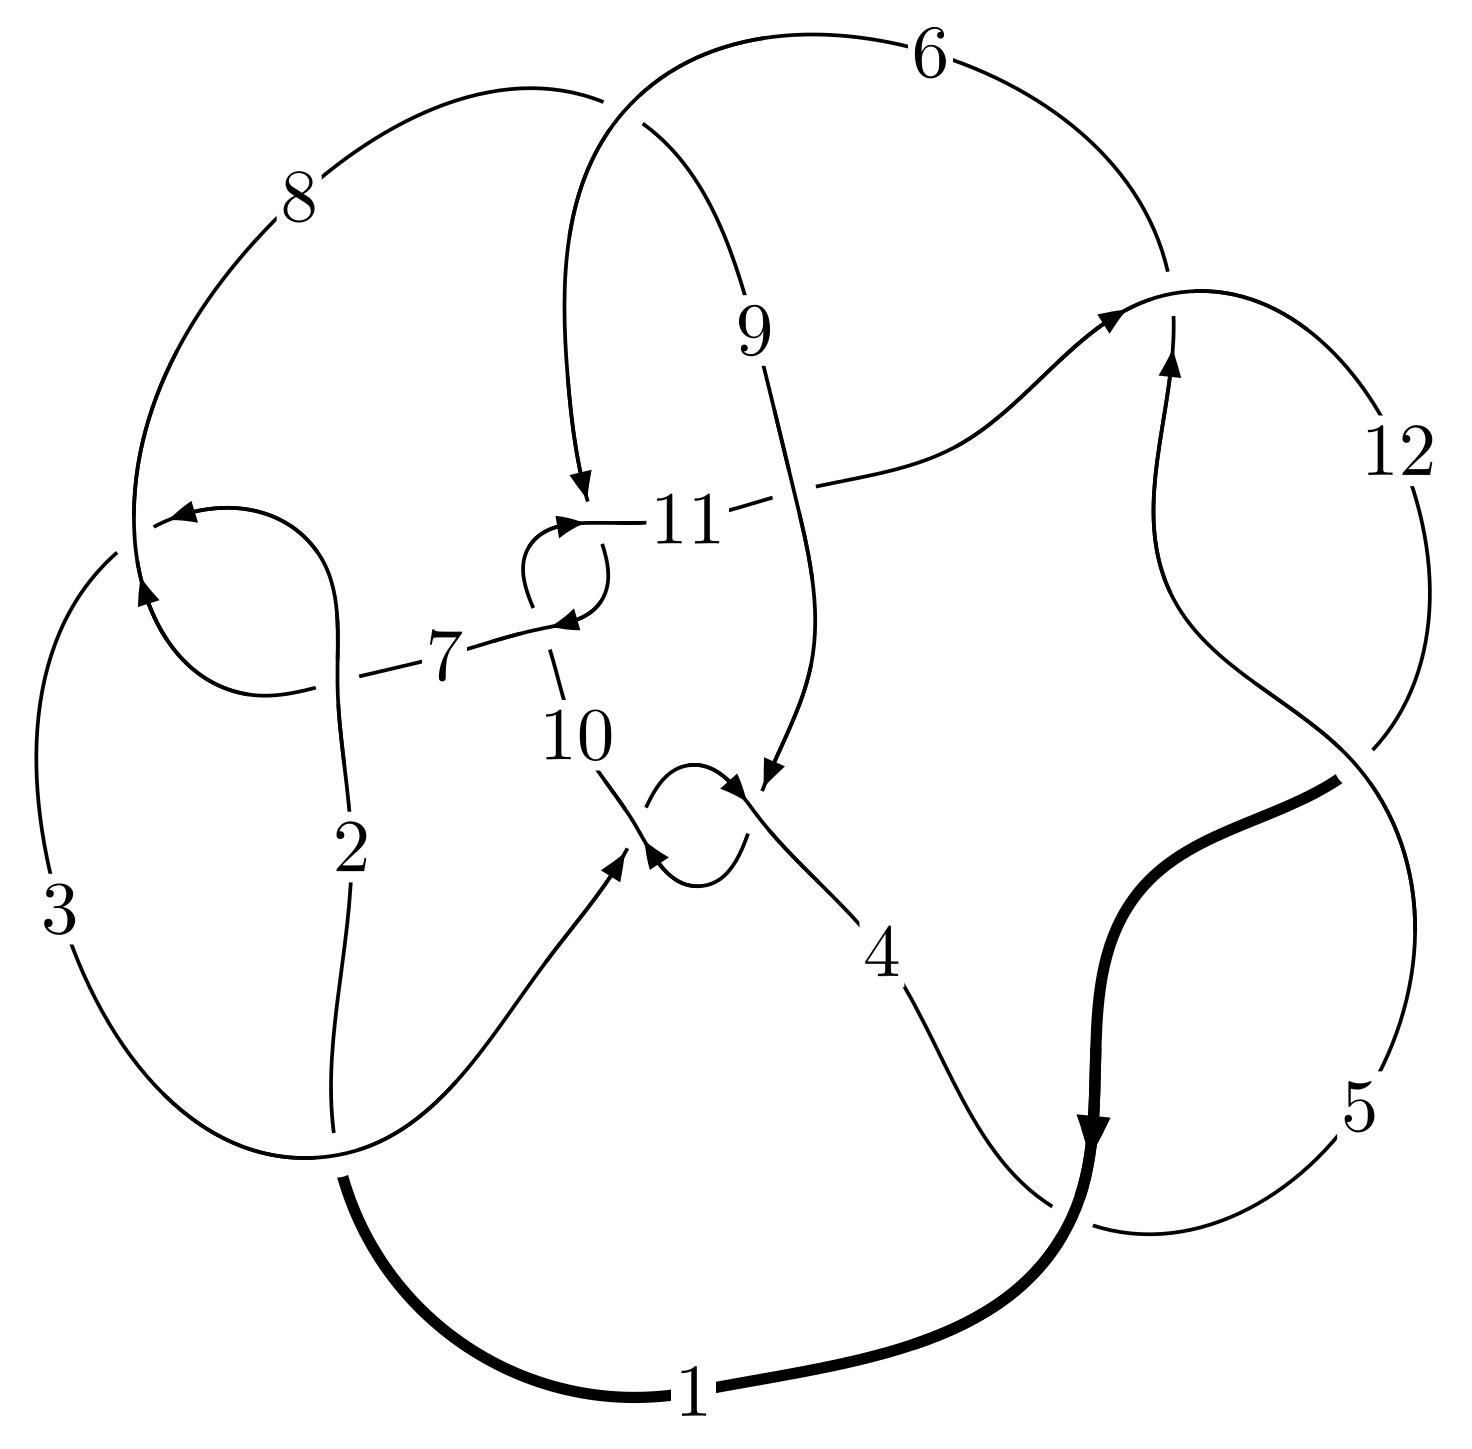
\includegraphics[width=112pt]{../../../GIT/diagram.site/Diagrams/png/1584_12a_0783.png}\\
\ \ \ A knot diagram\footnotemark}&
\allowdisplaybreaks
\textbf{Linearized knot diagam} \\
\cline{2-2}
 &
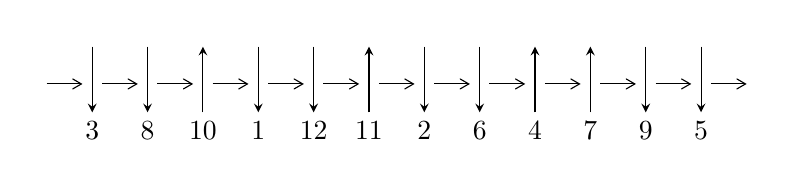
\begin{tikzpicture}[x=20pt, y=17pt]
	% nodes
	\node (C0) at (0, 0) {};
	\node (C1) at (1, 0) {};
	\node (C1U) at (1, +1) {};
	\node (C1D) at (1, -1) {3};

	\node (C2) at (2, 0) {};
	\node (C2U) at (2, +1) {};
	\node (C2D) at (2, -1) {8};

	\node (C3) at (3, 0) {};
	\node (C3U) at (3, +1) {};
	\node (C3D) at (3, -1) {10};

	\node (C4) at (4, 0) {};
	\node (C4U) at (4, +1) {};
	\node (C4D) at (4, -1) {1};

	\node (C5) at (5, 0) {};
	\node (C5U) at (5, +1) {};
	\node (C5D) at (5, -1) {12};

	\node (C6) at (6, 0) {};
	\node (C6U) at (6, +1) {};
	\node (C6D) at (6, -1) {11};

	\node (C7) at (7, 0) {};
	\node (C7U) at (7, +1) {};
	\node (C7D) at (7, -1) {2};

	\node (C8) at (8, 0) {};
	\node (C8U) at (8, +1) {};
	\node (C8D) at (8, -1) {6};

	\node (C9) at (9, 0) {};
	\node (C9U) at (9, +1) {};
	\node (C9D) at (9, -1) {4};

	\node (C10) at (10, 0) {};
	\node (C10U) at (10, +1) {};
	\node (C10D) at (10, -1) {7};

	\node (C11) at (11, 0) {};
	\node (C11U) at (11, +1) {};
	\node (C11D) at (11, -1) {9};

	\node (C12) at (12, 0) {};
	\node (C12U) at (12, +1) {};
	\node (C12D) at (12, -1) {5};
	\node (C13) at (13, 0) {};

	% arrows
	\draw[->,>={angle 60}]
	(C0) edge (C1) (C1) edge (C2) (C2) edge (C3) (C3) edge (C4) (C4) edge (C5) (C5) edge (C6) (C6) edge (C7) (C7) edge (C8) (C8) edge (C9) (C9) edge (C10) (C10) edge (C11) (C11) edge (C12) (C12) edge (C13) ;	\draw[->,>=stealth]
	(C1U) edge (C1D) (C2U) edge (C2D) (C3D) edge (C3U) (C4U) edge (C4D) (C5U) edge (C5D) (C6D) edge (C6U) (C7U) edge (C7D) (C8U) edge (C8D) (C9D) edge (C9U) (C10D) edge (C10U) (C11U) edge (C11D) (C12U) edge (C12D) ;
	\end{tikzpicture} \\
\hhline{~~} \\& 
\textbf{Solving Sequence} \\ \cline{2-2} 
 &
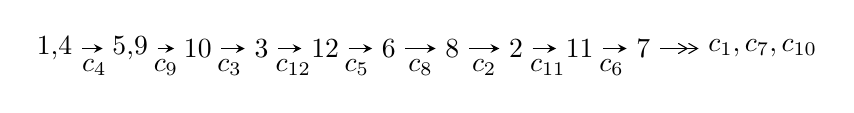
\begin{tikzpicture}[x=23pt, y=7pt]
	% node
	\node (A0) at (-1/8, 0) {1,4};
	\node (A1) at (17/16, 0) {5,9};
	\node (A2) at (17/8, 0) {10};
	\node (A3) at (25/8, 0) {3};
	\node (A4) at (33/8, 0) {12};
	\node (A5) at (41/8, 0) {6};
	\node (A6) at (49/8, 0) {8};
	\node (A7) at (57/8, 0) {2};
	\node (A8) at (65/8, 0) {11};
	\node (A9) at (73/8, 0) {7};
	\node (C1) at (1/2, -1) {$c_{4}$};
	\node (C2) at (13/8, -1) {$c_{9}$};
	\node (C3) at (21/8, -1) {$c_{3}$};
	\node (C4) at (29/8, -1) {$c_{12}$};
	\node (C5) at (37/8, -1) {$c_{5}$};
	\node (C6) at (45/8, -1) {$c_{8}$};
	\node (C7) at (53/8, -1) {$c_{2}$};
	\node (C8) at (61/8, -1) {$c_{11}$};
	\node (C9) at (69/8, -1) {$c_{6}$};
	\node (A10) at (11, 0) {$c_{1},c_{7},c_{10}$};

	% edge
	\draw[->,>=stealth]	
	(A0) edge (A1) (A1) edge (A2) (A2) edge (A3) (A3) edge (A4) (A4) edge (A5) (A5) edge (A6) (A6) edge (A7) (A7) edge (A8) (A8) edge (A9) ;
	\draw[->>,>={angle 60}]	
	(A9) edge (A10);
\end{tikzpicture} \\ 

\end{tabular} \\

\footnotetext{
The image of knot diagram is generated by the software ``\textbf{Draw programme}" developed by Andrew Bartholomew(\url{http://www.layer8.co.uk/maths/draw/index.htm\#Running-draw}), where we modified some parts for our purpose(\url{https://github.com/CATsTAILs/LinksPainter}).
}\phantom \\ \newline 
\centering \textbf{Ideals for irreducible components\footnotemark of $X_{\text{par}}$} 
 
\begin{align*}
I^u_{1}&=\langle 
1.66774\times10^{316} u^{116}-4.81256\times10^{316} u^{115}+\cdots+3.09892\times10^{315} b-8.67721\times10^{316},\\
\phantom{I^u_{1}}&\phantom{= \langle  }-4.47324\times10^{316} u^{116}+1.35366\times10^{317} u^{115}+\cdots+3.09892\times10^{315} a+4.03023\times10^{317},\\
\phantom{I^u_{1}}&\phantom{= \langle  }u^{117}-3 u^{116}+\cdots-33 u+1\rangle \\
I^u_{2}&=\langle 
-1685 u^{23}-3592 u^{22}+\cdots+1939 b+1461,\;337 u^{23}+663 u^{22}+\cdots+277 a+151,\\
\phantom{I^u_{2}}&\phantom{= \langle  }u^{24}+2 u^{23}+\cdots+6 u^2+1\rangle \\
\\
\end{align*}
\raggedright * 2 irreducible components of $\dim_{\mathbb{C}}=0$, with total 141 representations.\\
\footnotetext{All coefficients of polynomials are rational numbers. But the coefficients are sometimes approximated in decimal forms when there is not enough margin.}
\newpage
\renewcommand{\arraystretch}{1}
\centering \section*{I. $I^u_{1}= \langle 1.67\times10^{316} u^{116}-4.81\times10^{316} u^{115}+\cdots+3.10\times10^{315} b-8.68\times10^{316},\;-4.47\times10^{316} u^{116}+1.35\times10^{317} u^{115}+\cdots+3.10\times10^{315} a+4.03\times10^{317},\;u^{117}-3 u^{116}+\cdots-33 u+1 \rangle$}
\flushleft \textbf{(i) Arc colorings}\\
\begin{tabular}{m{7pt} m{180pt} m{7pt} m{180pt} }
\flushright $a_{1}=$&$\begin{pmatrix}0\\u\end{pmatrix}$ \\
\flushright $a_{4}=$&$\begin{pmatrix}1\\0\end{pmatrix}$ \\
\flushright $a_{5}=$&$\begin{pmatrix}1\\u^2\end{pmatrix}$ \\
\flushright $a_{9}=$&$\begin{pmatrix}14.4348 u^{116}-43.6818 u^{115}+\cdots+3655.33 u-130.053\\-5.38168 u^{116}+15.5298 u^{115}+\cdots-795.950 u+28.0008\end{pmatrix}$ \\
\flushright $a_{10}=$&$\begin{pmatrix}9.05317 u^{116}-28.1520 u^{115}+\cdots+2859.38 u-102.052\\-5.38168 u^{116}+15.5298 u^{115}+\cdots-795.950 u+28.0008\end{pmatrix}$ \\
\flushright $a_{3}=$&$\begin{pmatrix}18.3661 u^{116}-51.0532 u^{115}+\cdots+1634.41 u-43.2854\\-1.27374 u^{116}+2.87521 u^{115}+\cdots+377.420 u-16.6565\end{pmatrix}$ \\
\flushright $a_{12}=$&$\begin{pmatrix}u\\u^3+u\end{pmatrix}$ \\
\flushright $a_{6}=$&$\begin{pmatrix}u^2+1\\u^4+2 u^2\end{pmatrix}$ \\
\flushright $a_{8}=$&$\begin{pmatrix}10.0940 u^{116}-30.7903 u^{115}+\cdots+2861.66 u-100.955\\-5.31587 u^{116}+15.3684 u^{115}+\cdots-824.059 u+29.1264\end{pmatrix}$ \\
\flushright $a_{2}=$&$\begin{pmatrix}23.3386 u^{116}-66.6870 u^{115}+\cdots+3567.43 u-123.462\\4.20132 u^{116}-12.3487 u^{115}+\cdots+1036.39 u-37.7570\end{pmatrix}$ \\
\flushright $a_{11}=$&$\begin{pmatrix}17.6230 u^{116}-50.8082 u^{115}+\cdots+3952.88 u-154.468\\6.09960 u^{116}-17.2854 u^{115}+\cdots+682.688 u-21.1410\end{pmatrix}$ \\
\flushright $a_{7}=$&$\begin{pmatrix}-27.0752 u^{116}+76.3531 u^{115}+\cdots-3792.58 u+122.109\\0.611424 u^{116}-1.00040 u^{115}+\cdots-120.824 u+4.62257\end{pmatrix}$\\&\end{tabular}
\flushleft \textbf{(ii) Obstruction class $= -1$}\\~\\
\flushleft \textbf{(iii) Cusp Shapes $= 12.7365 u^{116}-40.8301 u^{115}+\cdots+4568.87 u-176.087$}\\~\\
\newpage\renewcommand{\arraystretch}{1}
\flushleft \textbf{(iv) u-Polynomials at the component}\newline \\
\begin{tabular}{m{50pt}|m{274pt}}
Crossings & \hspace{64pt}u-Polynomials at each crossing \\
\hline $$\begin{aligned}c_{1}\end{aligned}$$&$\begin{aligned}
&u^{117}+53 u^{116}+\cdots+10193283 u+534361
\end{aligned}$\\
\hline $$\begin{aligned}c_{2},c_{7}\end{aligned}$$&$\begin{aligned}
&u^{117}+u^{116}+\cdots+2625 u+731
\end{aligned}$\\
\hline $$\begin{aligned}c_{3},c_{9}\end{aligned}$$&$\begin{aligned}
&u^{117}+u^{116}+\cdots-3840 u+7424
\end{aligned}$\\
\hline $$\begin{aligned}c_{4},c_{5},c_{12}\end{aligned}$$&$\begin{aligned}
&u^{117}-3 u^{116}+\cdots-33 u+1
\end{aligned}$\\
\hline $$\begin{aligned}c_{6},c_{10}\end{aligned}$$&$\begin{aligned}
&u^{117}+43 u^{115}+\cdots+49298 u+2983
\end{aligned}$\\
\hline $$\begin{aligned}c_{8}\end{aligned}$$&$\begin{aligned}
&u^{117}-8 u^{116}+\cdots-336 u+32
\end{aligned}$\\
\hline $$\begin{aligned}c_{11}\end{aligned}$$&$\begin{aligned}
&u^{117}-3 u^{116}+\cdots+76 u-3
\end{aligned}$\\
\hline
\end{tabular}\\~\\
\newpage\renewcommand{\arraystretch}{1}
\flushleft \textbf{(v) Riley Polynomials at the component}\newline \\
\begin{tabular}{m{50pt}|m{274pt}}
Crossings & \hspace{64pt}Riley Polynomials at each crossing \\
\hline $$\begin{aligned}c_{1}\end{aligned}$$&$\begin{aligned}
&y^{117}+35 y^{116}+\cdots-9546989252781 y-285541678321
\end{aligned}$\\
\hline $$\begin{aligned}c_{2},c_{7}\end{aligned}$$&$\begin{aligned}
&y^{117}-53 y^{116}+\cdots+10193283 y-534361
\end{aligned}$\\
\hline $$\begin{aligned}c_{3},c_{9}\end{aligned}$$&$\begin{aligned}
&y^{117}+75 y^{116}+\cdots-1432518656 y-55115776
\end{aligned}$\\
\hline $$\begin{aligned}c_{4},c_{5},c_{12}\end{aligned}$$&$\begin{aligned}
&y^{117}+121 y^{116}+\cdots+91 y-1
\end{aligned}$\\
\hline $$\begin{aligned}c_{6},c_{10}\end{aligned}$$&$\begin{aligned}
&y^{117}+86 y^{116}+\cdots-304360514 y-8898289
\end{aligned}$\\
\hline $$\begin{aligned}c_{8}\end{aligned}$$&$\begin{aligned}
&y^{117}+22 y^{116}+\cdots-63744 y-1024
\end{aligned}$\\
\hline $$\begin{aligned}c_{11}\end{aligned}$$&$\begin{aligned}
&y^{117}-5 y^{116}+\cdots+526 y-9
\end{aligned}$\\
\hline
\end{tabular}\\~\\
\newpage\flushleft \textbf{(vi) Complex Volumes and Cusp Shapes}
$$\begin{array}{c|c|c}  
\text{Solutions to }I^u_{1}& \I (\text{vol} + \sqrt{-1}CS) & \text{Cusp shape}\\
 \hline 
\begin{aligned}
u &= -0.823621 + 0.550525 I \\
a &= \phantom{-}0.879159 - 0.328519 I \\
b &= -0.467634 - 1.204290 I\end{aligned}
 & -3.41835 + 7.95463 I & \phantom{-0.000000 } 0 \\ \hline\begin{aligned}
u &= -0.823621 - 0.550525 I \\
a &= \phantom{-}0.879159 + 0.328519 I \\
b &= -0.467634 + 1.204290 I\end{aligned}
 & -3.41835 - 7.95463 I & \phantom{-0.000000 } 0 \\ \hline\begin{aligned}
u &= \phantom{-}0.894141 + 0.511446 I \\
a &= -0.780617 - 0.519456 I \\
b &= \phantom{-}0.58826 - 1.31392 I\end{aligned}
 & -5.7687 - 13.7661 I & \phantom{-0.000000 } 0 \\ \hline\begin{aligned}
u &= \phantom{-}0.894141 - 0.511446 I \\
a &= -0.780617 + 0.519456 I \\
b &= \phantom{-}0.58826 + 1.31392 I\end{aligned}
 & -5.7687 + 13.7661 I & \phantom{-0.000000 } 0 \\ \hline\begin{aligned}
u &= -0.884123 + 0.552686 I \\
a &= -0.507230 + 0.478718 I \\
b &= \phantom{-}0.427383 + 0.938946 I\end{aligned}
 & \phantom{-}0.49446 + 2.31225 I & \phantom{-0.000000 } 0 \\ \hline\begin{aligned}
u &= -0.884123 - 0.552686 I \\
a &= -0.507230 - 0.478718 I \\
b &= \phantom{-}0.427383 - 0.938946 I\end{aligned}
 & \phantom{-}0.49446 - 2.31225 I & \phantom{-0.000000 } 0 \\ \hline\begin{aligned}
u &= -0.884826 + 0.567387 I \\
a &= \phantom{-}0.382268 + 0.016594 I \\
b &= \phantom{-}0.213689 - 1.041540 I\end{aligned}
 & -3.41075 - 2.38257 I & \phantom{-0.000000 } 0 \\ \hline\begin{aligned}
u &= -0.884826 - 0.567387 I \\
a &= \phantom{-}0.382268 - 0.016594 I \\
b &= \phantom{-}0.213689 + 1.041540 I\end{aligned}
 & -3.41075 + 2.38257 I & \phantom{-0.000000 } 0 \\ \hline\begin{aligned}
u &= \phantom{-}0.903111 + 0.107618 I \\
a &= \phantom{-}0.570322 + 0.901913 I \\
b &= \phantom{-}0.071397 + 0.951586 I\end{aligned}
 & -2.61957 - 1.38881 I & \phantom{-0.000000 } 0 \\ \hline\begin{aligned}
u &= \phantom{-}0.903111 - 0.107618 I \\
a &= \phantom{-}0.570322 - 0.901913 I \\
b &= \phantom{-}0.071397 - 0.951586 I\end{aligned}
 & -2.61957 + 1.38881 I & \phantom{-0.000000 } 0\\
 \hline 
 \end{array}$$\newpage$$\begin{array}{c|c|c}  
\text{Solutions to }I^u_{1}& \I (\text{vol} + \sqrt{-1}CS) & \text{Cusp shape}\\
 \hline 
\begin{aligned}
u &= -0.543248 + 0.726897 I \\
a &= \phantom{-}0.023976 + 0.258840 I \\
b &= -0.482842 + 0.201823 I\end{aligned}
 & \phantom{-}1.76136 + 3.29242 I & \phantom{-0.000000 } 0 \\ \hline\begin{aligned}
u &= -0.543248 - 0.726897 I \\
a &= \phantom{-}0.023976 - 0.258840 I \\
b &= -0.482842 - 0.201823 I\end{aligned}
 & \phantom{-}1.76136 - 3.29242 I & \phantom{-0.000000 } 0 \\ \hline\begin{aligned}
u &= \phantom{-}0.109290 + 1.108720 I \\
a &= \phantom{-}0.049329 - 0.395592 I \\
b &= \phantom{-}0.292744 + 1.122070 I\end{aligned}
 & -0.596112 + 0.807380 I & \phantom{-0.000000 } 0 \\ \hline\begin{aligned}
u &= \phantom{-}0.109290 - 1.108720 I \\
a &= \phantom{-}0.049329 + 0.395592 I \\
b &= \phantom{-}0.292744 - 1.122070 I\end{aligned}
 & -0.596112 - 0.807380 I & \phantom{-0.000000 } 0 \\ \hline\begin{aligned}
u &= \phantom{-}0.514267 + 0.720818 I \\
a &= -0.464389 + 0.032530 I \\
b &= -0.09329 - 1.46240 I\end{aligned}
 & -8.74988 + 0.47669 I & \phantom{-0.000000 } 0 \\ \hline\begin{aligned}
u &= \phantom{-}0.514267 - 0.720818 I \\
a &= -0.464389 - 0.032530 I \\
b &= -0.09329 + 1.46240 I\end{aligned}
 & -8.74988 - 0.47669 I & \phantom{-0.000000 } 0 \\ \hline\begin{aligned}
u &= \phantom{-}1.033930 + 0.438997 I \\
a &= \phantom{-}0.423742 + 0.626882 I \\
b &= -0.406738 + 1.124730 I\end{aligned}
 & -0.83319 - 6.95313 I & \phantom{-0.000000 } 0 \\ \hline\begin{aligned}
u &= \phantom{-}1.033930 - 0.438997 I \\
a &= \phantom{-}0.423742 - 0.626882 I \\
b &= -0.406738 - 1.124730 I\end{aligned}
 & -0.83319 + 6.95313 I & \phantom{-0.000000 } 0 \\ \hline\begin{aligned}
u &= -0.335464 + 0.800015 I \\
a &= \phantom{-}0.72265 + 1.29877 I \\
b &= \phantom{-}0.060176 - 1.119970 I\end{aligned}
 & -1.45414 + 2.96537 I & \phantom{-0.000000 } 0 \\ \hline\begin{aligned}
u &= -0.335464 - 0.800015 I \\
a &= \phantom{-}0.72265 - 1.29877 I \\
b &= \phantom{-}0.060176 + 1.119970 I\end{aligned}
 & -1.45414 - 2.96537 I & \phantom{-0.000000 } 0\\
 \hline 
 \end{array}$$\newpage$$\begin{array}{c|c|c}  
\text{Solutions to }I^u_{1}& \I (\text{vol} + \sqrt{-1}CS) & \text{Cusp shape}\\
 \hline 
\begin{aligned}
u &= \phantom{-}0.927366 + 0.715486 I \\
a &= -0.396497 + 0.077797 I \\
b &= -0.424770 - 1.119600 I\end{aligned}
 & -5.27147 + 7.80861 I & \phantom{-0.000000 } 0 \\ \hline\begin{aligned}
u &= \phantom{-}0.927366 - 0.715486 I \\
a &= -0.396497 - 0.077797 I \\
b &= -0.424770 + 1.119600 I\end{aligned}
 & -5.27147 - 7.80861 I & \phantom{-0.000000 } 0 \\ \hline\begin{aligned}
u &= \phantom{-}0.179005 + 1.161270 I \\
a &= -0.014852 + 1.362400 I \\
b &= -0.34866 - 1.47737 I\end{aligned}
 & -2.10538 + 2.69369 I & \phantom{-0.000000 } 0 \\ \hline\begin{aligned}
u &= \phantom{-}0.179005 - 1.161270 I \\
a &= -0.014852 - 1.362400 I \\
b &= -0.34866 + 1.47737 I\end{aligned}
 & -2.10538 - 2.69369 I & \phantom{-0.000000 } 0 \\ \hline\begin{aligned}
u &= \phantom{-}0.686090 + 0.410531 I \\
a &= -1.52456 - 0.48044 I \\
b &= \phantom{-}0.208285 - 1.343460 I\end{aligned}
 & -9.63014 - 4.71202 I & \phantom{-0.000000 } 0 \\ \hline\begin{aligned}
u &= \phantom{-}0.686090 - 0.410531 I \\
a &= -1.52456 + 0.48044 I \\
b &= \phantom{-}0.208285 + 1.343460 I\end{aligned}
 & -9.63014 + 4.71202 I & \phantom{-0.000000 } 0 \\ \hline\begin{aligned}
u &= -0.731192 + 0.191208 I \\
a &= -0.529894 - 1.236080 I \\
b &= -0.488545 - 0.420301 I\end{aligned}
 & -3.04512 - 4.06095 I & \phantom{-0.000000 } 0 \\ \hline\begin{aligned}
u &= -0.731192 - 0.191208 I \\
a &= -0.529894 + 1.236080 I \\
b &= -0.488545 + 0.420301 I\end{aligned}
 & -3.04512 + 4.06095 I & \phantom{-0.000000 } 0 \\ \hline\begin{aligned}
u &= \phantom{-}0.183580 + 0.718841 I \\
a &= -0.293362 + 0.722372 I \\
b &= \phantom{-}0.503030 + 0.203505 I\end{aligned}
 & \phantom{-}2.15124 + 1.14844 I & \phantom{-0.000000 } 0 \\ \hline\begin{aligned}
u &= \phantom{-}0.183580 - 0.718841 I \\
a &= -0.293362 - 0.722372 I \\
b &= \phantom{-}0.503030 - 0.203505 I\end{aligned}
 & \phantom{-}2.15124 - 1.14844 I & \phantom{-0.000000 } 0\\
 \hline 
 \end{array}$$\newpage$$\begin{array}{c|c|c}  
\text{Solutions to }I^u_{1}& \I (\text{vol} + \sqrt{-1}CS) & \text{Cusp shape}\\
 \hline 
\begin{aligned}
u &= -0.402505 + 0.600498 I \\
a &= \phantom{-}0.073364 - 1.195060 I \\
b &= -0.704880 + 0.467391 I\end{aligned}
 & -2.29151 + 2.22633 I & \phantom{-0.000000 } 0 \\ \hline\begin{aligned}
u &= -0.402505 - 0.600498 I \\
a &= \phantom{-}0.073364 + 1.195060 I \\
b &= -0.704880 - 0.467391 I\end{aligned}
 & -2.29151 - 2.22633 I & \phantom{-0.000000 } 0 \\ \hline\begin{aligned}
u &= -0.510980 + 0.511223 I \\
a &= -0.329365 - 0.168857 I \\
b &= \phantom{-}1.145480 - 0.040555 I\end{aligned}
 & -1.89926 + 7.77304 I & \phantom{-0.000000 } 0 \\ \hline\begin{aligned}
u &= -0.510980 - 0.511223 I \\
a &= -0.329365 + 0.168857 I \\
b &= \phantom{-}1.145480 + 0.040555 I\end{aligned}
 & -1.89926 - 7.77304 I & \phantom{-0.000000 } 0 \\ \hline\begin{aligned}
u &= -0.031981 + 1.295900 I \\
a &= \phantom{-}1.91372 - 0.25329 I \\
b &= -0.004589 + 0.595418 I\end{aligned}
 & -0.49033 + 6.08864 I & \phantom{-0.000000 } 0 \\ \hline\begin{aligned}
u &= -0.031981 - 1.295900 I \\
a &= \phantom{-}1.91372 + 0.25329 I \\
b &= -0.004589 - 0.595418 I\end{aligned}
 & -0.49033 - 6.08864 I & \phantom{-0.000000 } 0 \\ \hline\begin{aligned}
u &= -0.631032 + 0.299385 I \\
a &= -0.577972 + 0.611171 I \\
b &= \phantom{-}0.979166 + 0.564250 I\end{aligned}
 & -3.34894 + 1.33915 I & \phantom{-0.000000 } 0 \\ \hline\begin{aligned}
u &= -0.631032 - 0.299385 I \\
a &= -0.577972 - 0.611171 I \\
b &= \phantom{-}0.979166 - 0.564250 I\end{aligned}
 & -3.34894 - 1.33915 I & \phantom{-0.000000 } 0 \\ \hline\begin{aligned}
u &= \phantom{-}0.005585 + 1.309210 I \\
a &= -1.47104 + 0.80161 I \\
b &= \phantom{-}0.333045 - 0.740450 I\end{aligned}
 & \phantom{-}1.98828 + 1.89618 I & \phantom{-0.000000 } 0 \\ \hline\begin{aligned}
u &= \phantom{-}0.005585 - 1.309210 I \\
a &= -1.47104 - 0.80161 I \\
b &= \phantom{-}0.333045 + 0.740450 I\end{aligned}
 & \phantom{-}1.98828 - 1.89618 I & \phantom{-0.000000 } 0\\
 \hline 
 \end{array}$$\newpage$$\begin{array}{c|c|c}  
\text{Solutions to }I^u_{1}& \I (\text{vol} + \sqrt{-1}CS) & \text{Cusp shape}\\
 \hline 
\begin{aligned}
u &= \phantom{-}0.154129 + 1.302490 I \\
a &= \phantom{-}2.25963 - 0.64816 I \\
b &= -1.18123 + 1.23666 I\end{aligned}
 & -1.44906 - 8.22432 I & \phantom{-0.000000 } 0 \\ \hline\begin{aligned}
u &= \phantom{-}0.154129 - 1.302490 I \\
a &= \phantom{-}2.25963 + 0.64816 I \\
b &= -1.18123 - 1.23666 I\end{aligned}
 & -1.44906 + 8.22432 I & \phantom{-0.000000 } 0 \\ \hline\begin{aligned}
u &= -0.650118 + 0.160046 I \\
a &= \phantom{-}0.434603 - 0.372811 I \\
b &= -0.487202 - 1.161570 I\end{aligned}
 & -3.58375 + 0.59174 I & \phantom{-0.000000 } 0 \\ \hline\begin{aligned}
u &= -0.650118 - 0.160046 I \\
a &= \phantom{-}0.434603 + 0.372811 I \\
b &= -0.487202 + 1.161570 I\end{aligned}
 & -3.58375 - 0.59174 I & \phantom{-0.000000 } 0 \\ \hline\begin{aligned}
u &= -0.172418 + 1.338520 I \\
a &= -1.67003 - 0.50766 I \\
b &= \phantom{-}0.91972 + 1.07639 I\end{aligned}
 & \phantom{-}1.04521 + 3.50568 I & \phantom{-0.000000 } 0 \\ \hline\begin{aligned}
u &= -0.172418 - 1.338520 I \\
a &= -1.67003 + 0.50766 I \\
b &= \phantom{-}0.91972 - 1.07639 I\end{aligned}
 & \phantom{-}1.04521 - 3.50568 I & \phantom{-0.000000 } 0 \\ \hline\begin{aligned}
u &= -0.297953 + 1.325140 I \\
a &= -0.970664 + 0.277028 I \\
b &= \phantom{-}0.481784 + 0.485463 I\end{aligned}
 & \phantom{-}2.47338 + 2.95926 I & \phantom{-0.000000 } 0 \\ \hline\begin{aligned}
u &= -0.297953 - 1.325140 I \\
a &= -0.970664 - 0.277028 I \\
b &= \phantom{-}0.481784 - 0.485463 I\end{aligned}
 & \phantom{-}2.47338 - 2.95926 I & \phantom{-0.000000 } 0 \\ \hline\begin{aligned}
u &= \phantom{-}0.101671 + 1.355120 I \\
a &= \phantom{-}1.32440 - 1.38228 I \\
b &= -0.65371 + 1.46359 I\end{aligned}
 & -3.00489 - 0.37587 I & \phantom{-0.000000 } 0 \\ \hline\begin{aligned}
u &= \phantom{-}0.101671 - 1.355120 I \\
a &= \phantom{-}1.32440 + 1.38228 I \\
b &= -0.65371 - 1.46359 I\end{aligned}
 & -3.00489 + 0.37587 I & \phantom{-0.000000 } 0\\
 \hline 
 \end{array}$$\newpage$$\begin{array}{c|c|c}  
\text{Solutions to }I^u_{1}& \I (\text{vol} + \sqrt{-1}CS) & \text{Cusp shape}\\
 \hline 
\begin{aligned}
u &= \phantom{-}0.521043 + 1.261250 I \\
a &= \phantom{-}0.576159 + 0.158488 I \\
b &= \phantom{-}0.151512 + 0.745889 I\end{aligned}
 & \phantom{-}1.74357 + 0.70351 I & \phantom{-0.000000 } 0 \\ \hline\begin{aligned}
u &= \phantom{-}0.521043 - 1.261250 I \\
a &= \phantom{-}0.576159 - 0.158488 I \\
b &= \phantom{-}0.151512 - 0.745889 I\end{aligned}
 & \phantom{-}1.74357 - 0.70351 I & \phantom{-0.000000 } 0 \\ \hline\begin{aligned}
u &= \phantom{-}0.042813 + 1.366880 I \\
a &= \phantom{-}0.01714 + 1.46662 I \\
b &= -0.16031 - 2.18447 I\end{aligned}
 & -3.54384 - 1.70880 I & \phantom{-0.000000 } 0 \\ \hline\begin{aligned}
u &= \phantom{-}0.042813 - 1.366880 I \\
a &= \phantom{-}0.01714 - 1.46662 I \\
b &= -0.16031 + 2.18447 I\end{aligned}
 & -3.54384 + 1.70880 I & \phantom{-0.000000 } 0 \\ \hline\begin{aligned}
u &= -0.322206 + 0.536631 I \\
a &= -1.016520 - 0.150138 I \\
b &= \phantom{-}0.304603 + 0.787145 I\end{aligned}
 & -0.33317 + 1.47731 I & -4.00000 - 3.46903 I \\ \hline\begin{aligned}
u &= -0.322206 - 0.536631 I \\
a &= -1.016520 + 0.150138 I \\
b &= \phantom{-}0.304603 - 0.787145 I\end{aligned}
 & -0.33317 - 1.47731 I & -4.00000 + 3.46903 I \\ \hline\begin{aligned}
u &= \phantom{-}0.189917 + 1.373320 I \\
a &= -1.95190 + 0.28181 I \\
b &= \phantom{-}0.718301 - 1.009000 I\end{aligned}
 & \phantom{-}1.51558 - 6.19254 I & \phantom{-0.000000 } 0 \\ \hline\begin{aligned}
u &= \phantom{-}0.189917 - 1.373320 I \\
a &= -1.95190 - 0.28181 I \\
b &= \phantom{-}0.718301 + 1.009000 I\end{aligned}
 & \phantom{-}1.51558 + 6.19254 I & \phantom{-0.000000 } 0 \\ \hline\begin{aligned}
u &= \phantom{-}0.285517 + 1.363260 I \\
a &= -1.49773 - 0.07523 I \\
b &= \phantom{-}0.295518 - 0.750349 I\end{aligned}
 & \phantom{-}2.06044 - 5.45428 I & \phantom{-0.000000 } 0 \\ \hline\begin{aligned}
u &= \phantom{-}0.285517 - 1.363260 I \\
a &= -1.49773 + 0.07523 I \\
b &= \phantom{-}0.295518 + 0.750349 I\end{aligned}
 & \phantom{-}2.06044 + 5.45428 I & \phantom{-0.000000 } 0\\
 \hline 
 \end{array}$$\newpage$$\begin{array}{c|c|c}  
\text{Solutions to }I^u_{1}& \I (\text{vol} + \sqrt{-1}CS) & \text{Cusp shape}\\
 \hline 
\begin{aligned}
u &= \phantom{-}0.067806 + 1.396920 I \\
a &= \phantom{-}0.835447 - 0.008036 I \\
b &= -0.26236 + 1.39556 I\end{aligned}
 & \phantom{-}3.07434 - 3.88441 I & \phantom{-0.000000 } 0 \\ \hline\begin{aligned}
u &= \phantom{-}0.067806 - 1.396920 I \\
a &= \phantom{-}0.835447 + 0.008036 I \\
b &= -0.26236 - 1.39556 I\end{aligned}
 & \phantom{-}3.07434 + 3.88441 I & \phantom{-0.000000 } 0 \\ \hline\begin{aligned}
u &= \phantom{-}0.000835 + 1.406560 I \\
a &= -1.346950 + 0.071829 I \\
b &= \phantom{-}0.425276 + 1.059150 I\end{aligned}
 & \phantom{-}4.92018 - 2.05187 I & \phantom{-0.000000 } 0 \\ \hline\begin{aligned}
u &= \phantom{-}0.000835 - 1.406560 I \\
a &= -1.346950 - 0.071829 I \\
b &= \phantom{-}0.425276 - 1.059150 I\end{aligned}
 & \phantom{-}4.92018 + 2.05187 I & \phantom{-0.000000 } 0 \\ \hline\begin{aligned}
u &= \phantom{-}0.571446 + 0.150027 I \\
a &= \phantom{-}0.98274 + 1.20657 I \\
b &= -0.519717 + 1.075700 I\end{aligned}
 & -3.33365 - 3.47759 I & -11.24105 + 4.72691 I \\ \hline\begin{aligned}
u &= \phantom{-}0.571446 - 0.150027 I \\
a &= \phantom{-}0.98274 - 1.20657 I \\
b &= -0.519717 - 1.075700 I\end{aligned}
 & -3.33365 + 3.47759 I & -11.24105 - 4.72691 I \\ \hline\begin{aligned}
u &= \phantom{-}0.589947 + 0.030203 I \\
a &= -0.393805 - 0.733976 I \\
b &= \phantom{-}0.75592 - 1.34795 I\end{aligned}
 & -5.52040 - 5.62216 I & -13.4525 + 5.1611 I \\ \hline\begin{aligned}
u &= \phantom{-}0.589947 - 0.030203 I \\
a &= -0.393805 + 0.733976 I \\
b &= \phantom{-}0.75592 + 1.34795 I\end{aligned}
 & -5.52040 + 5.62216 I & -13.4525 - 5.1611 I \\ \hline\begin{aligned}
u &= -0.23559 + 1.40990 I \\
a &= \phantom{-}1.89282 - 0.27860 I \\
b &= -1.213310 - 0.527341 I\end{aligned}
 & \phantom{-}2.10227 + 4.48694 I & \phantom{-0.000000 } 0 \\ \hline\begin{aligned}
u &= -0.23559 - 1.40990 I \\
a &= \phantom{-}1.89282 + 0.27860 I \\
b &= -1.213310 + 0.527341 I\end{aligned}
 & \phantom{-}2.10227 - 4.48694 I & \phantom{-0.000000 } 0\\
 \hline 
 \end{array}$$\newpage$$\begin{array}{c|c|c}  
\text{Solutions to }I^u_{1}& \I (\text{vol} + \sqrt{-1}CS) & \text{Cusp shape}\\
 \hline 
\begin{aligned}
u &= -0.05326 + 1.43162 I \\
a &= \phantom{-}1.62952 + 0.38146 I \\
b &= -0.630137 - 0.915075 I\end{aligned}
 & \phantom{-}5.79734 + 2.20208 I & \phantom{-0.000000 } 0 \\ \hline\begin{aligned}
u &= -0.05326 - 1.43162 I \\
a &= \phantom{-}1.62952 - 0.38146 I \\
b &= -0.630137 + 0.915075 I\end{aligned}
 & \phantom{-}5.79734 - 2.20208 I & \phantom{-0.000000 } 0 \\ \hline\begin{aligned}
u &= \phantom{-}0.10086 + 1.43008 I \\
a &= -1.83472 - 0.17438 I \\
b &= \phantom{-}0.494211 - 1.188990 I\end{aligned}
 & \phantom{-}1.80679 - 7.97564 I & \phantom{-0.000000 } 0 \\ \hline\begin{aligned}
u &= \phantom{-}0.10086 - 1.43008 I \\
a &= -1.83472 + 0.17438 I \\
b &= \phantom{-}0.494211 + 1.188990 I\end{aligned}
 & \phantom{-}1.80679 + 7.97564 I & \phantom{-0.000000 } 0 \\ \hline\begin{aligned}
u &= \phantom{-}0.392829 + 0.395363 I \\
a &= \phantom{-}0.972048 - 0.353878 I \\
b &= -0.862074 - 0.089310 I\end{aligned}
 & -0.01409 - 3.27867 I & -1.12600 + 4.52290 I \\ \hline\begin{aligned}
u &= \phantom{-}0.392829 - 0.395363 I \\
a &= \phantom{-}0.972048 + 0.353878 I \\
b &= -0.862074 + 0.089310 I\end{aligned}
 & -0.01409 + 3.27867 I & -1.12600 - 4.52290 I \\ \hline\begin{aligned}
u &= -0.526645\phantom{ +0.000000I} \\
a &= \phantom{-}0.170705\phantom{ +0.000000I} \\
b &= -0.396012\phantom{ +0.000000I}\end{aligned}
 & -1.22542\phantom{ +0.000000I} & -7.59440\phantom{ +0.000000I} \\ \hline\begin{aligned}
u &= \phantom{-}0.14747 + 1.47198 I \\
a &= -1.60654 - 0.38950 I \\
b &= \phantom{-}1.256990 + 0.425301 I\end{aligned}
 & \phantom{-}6.13929 - 5.31752 I & \phantom{-0.000000 } 0 \\ \hline\begin{aligned}
u &= \phantom{-}0.14747 - 1.47198 I \\
a &= -1.60654 + 0.38950 I \\
b &= \phantom{-}1.256990 - 0.425301 I\end{aligned}
 & \phantom{-}6.13929 + 5.31752 I & \phantom{-0.000000 } 0 \\ \hline\begin{aligned}
u &= \phantom{-}0.23432 + 1.48664 I \\
a &= \phantom{-}1.68860 - 0.71078 I \\
b &= -0.352886 + 1.212040 I\end{aligned}
 & -3.44609 - 8.03987 I & \phantom{-0.000000 } 0\\
 \hline 
 \end{array}$$\newpage$$\begin{array}{c|c|c}  
\text{Solutions to }I^u_{1}& \I (\text{vol} + \sqrt{-1}CS) & \text{Cusp shape}\\
 \hline 
\begin{aligned}
u &= \phantom{-}0.23432 - 1.48664 I \\
a &= \phantom{-}1.68860 + 0.71078 I \\
b &= -0.352886 - 1.212040 I\end{aligned}
 & -3.44609 + 8.03987 I & \phantom{-0.000000 } 0 \\ \hline\begin{aligned}
u &= -0.18985 + 1.49347 I \\
a &= \phantom{-}1.67005 - 0.47304 I \\
b &= -1.56712 + 0.24896 I\end{aligned}
 & \phantom{-}4.61397 + 10.40970 I & \phantom{-0.000000 } 0 \\ \hline\begin{aligned}
u &= -0.18985 - 1.49347 I \\
a &= \phantom{-}1.67005 + 0.47304 I \\
b &= -1.56712 - 0.24896 I\end{aligned}
 & \phantom{-}4.61397 - 10.40970 I & \phantom{-0.000000 } 0 \\ \hline\begin{aligned}
u &= -0.08394 + 1.52109 I \\
a &= \phantom{-}1.35057 + 0.74054 I \\
b &= -0.619107 - 0.668117 I\end{aligned}
 & \phantom{-}6.46201 + 2.72953 I & \phantom{-0.000000 } 0 \\ \hline\begin{aligned}
u &= -0.08394 - 1.52109 I \\
a &= \phantom{-}1.35057 - 0.74054 I \\
b &= -0.619107 + 0.668117 I\end{aligned}
 & \phantom{-}6.46201 - 2.72953 I & \phantom{-0.000000 } 0 \\ \hline\begin{aligned}
u &= \phantom{-}0.11844 + 1.53057 I \\
a &= \phantom{-}1.220390 + 0.284829 I \\
b &= -1.039580 - 0.406581 I\end{aligned}
 & \phantom{-}9.51686 - 0.34246 I & \phantom{-0.000000 } 0 \\ \hline\begin{aligned}
u &= \phantom{-}0.11844 - 1.53057 I \\
a &= \phantom{-}1.220390 - 0.284829 I \\
b &= -1.039580 + 0.406581 I\end{aligned}
 & \phantom{-}9.51686 + 0.34246 I & \phantom{-0.000000 } 0 \\ \hline\begin{aligned}
u &= -0.18396 + 1.53942 I \\
a &= -1.126870 + 0.247647 I \\
b &= \phantom{-}1.014630 - 0.185823 I\end{aligned}
 & \phantom{-}9.06433 + 6.00935 I & \phantom{-0.000000 } 0 \\ \hline\begin{aligned}
u &= -0.18396 - 1.53942 I \\
a &= -1.126870 - 0.247647 I \\
b &= \phantom{-}1.014630 + 0.185823 I\end{aligned}
 & \phantom{-}9.06433 - 6.00935 I & \phantom{-0.000000 } 0 \\ \hline\begin{aligned}
u &= -0.29207 + 1.53254 I \\
a &= \phantom{-}1.367380 + 0.203140 I \\
b &= -0.689755 - 1.149300 I\end{aligned}
 & \phantom{-}7.22273 + 6.49045 I & \phantom{-0.000000 } 0\\
 \hline 
 \end{array}$$\newpage$$\begin{array}{c|c|c}  
\text{Solutions to }I^u_{1}& \I (\text{vol} + \sqrt{-1}CS) & \text{Cusp shape}\\
 \hline 
\begin{aligned}
u &= -0.29207 - 1.53254 I \\
a &= \phantom{-}1.367380 - 0.203140 I \\
b &= -0.689755 + 1.149300 I\end{aligned}
 & \phantom{-}7.22273 - 6.49045 I & \phantom{-0.000000 } 0 \\ \hline\begin{aligned}
u &= -0.02699 + 1.56109 I \\
a &= -0.747730 + 0.563415 I \\
b &= \phantom{-}0.648365 - 0.091496 I\end{aligned}
 & \phantom{-}4.92005 + 3.52483 I & \phantom{-0.000000 } 0 \\ \hline\begin{aligned}
u &= -0.02699 - 1.56109 I \\
a &= -0.747730 - 0.563415 I \\
b &= \phantom{-}0.648365 + 0.091496 I\end{aligned}
 & \phantom{-}4.92005 - 3.52483 I & \phantom{-0.000000 } 0 \\ \hline\begin{aligned}
u &= \phantom{-}0.35127 + 1.52895 I \\
a &= -1.328450 + 0.150987 I \\
b &= \phantom{-}0.59330 - 1.30601 I\end{aligned}
 & \phantom{-}5.54664 - 11.83250 I & \phantom{-0.000000 } 0 \\ \hline\begin{aligned}
u &= \phantom{-}0.35127 - 1.52895 I \\
a &= -1.328450 - 0.150987 I \\
b &= \phantom{-}0.59330 + 1.30601 I\end{aligned}
 & \phantom{-}5.54664 + 11.83250 I & \phantom{-0.000000 } 0 \\ \hline\begin{aligned}
u &= \phantom{-}0.32370 + 1.53537 I \\
a &= \phantom{-}1.60596 - 0.34916 I \\
b &= -0.75234 + 1.41304 I\end{aligned}
 & \phantom{-}0.8424 - 18.2009 I & \phantom{-0.000000 } 0 \\ \hline\begin{aligned}
u &= \phantom{-}0.32370 - 1.53537 I \\
a &= \phantom{-}1.60596 + 0.34916 I \\
b &= -0.75234 - 1.41304 I\end{aligned}
 & \phantom{-}0.8424 + 18.2009 I & \phantom{-0.000000 } 0 \\ \hline\begin{aligned}
u &= -0.29178 + 1.54216 I \\
a &= -1.53508 - 0.42912 I \\
b &= \phantom{-}0.69158 + 1.25263 I\end{aligned}
 & \phantom{-}3.37954 + 12.04530 I & \phantom{-0.000000 } 0 \\ \hline\begin{aligned}
u &= -0.29178 - 1.54216 I \\
a &= -1.53508 + 0.42912 I \\
b &= \phantom{-}0.69158 - 1.25263 I\end{aligned}
 & \phantom{-}3.37954 - 12.04530 I & \phantom{-0.000000 } 0 \\ \hline\begin{aligned}
u &= -0.07201 + 1.58383 I \\
a &= -0.62713 - 1.46462 I \\
b &= \phantom{-}0.123823 + 0.804225 I\end{aligned}
 & \phantom{-}6.50048 + 4.26640 I & \phantom{-0.000000 } 0\\
 \hline 
 \end{array}$$\newpage$$\begin{array}{c|c|c}  
\text{Solutions to }I^u_{1}& \I (\text{vol} + \sqrt{-1}CS) & \text{Cusp shape}\\
 \hline 
\begin{aligned}
u &= -0.07201 - 1.58383 I \\
a &= -0.62713 + 1.46462 I \\
b &= \phantom{-}0.123823 - 0.804225 I\end{aligned}
 & \phantom{-}6.50048 - 4.26640 I & \phantom{-0.000000 } 0 \\ \hline\begin{aligned}
u &= \phantom{-}0.50977 + 1.50725 I \\
a &= \phantom{-}0.719688 + 0.014267 I \\
b &= -0.271664 + 1.229580 I\end{aligned}
 & \phantom{-}1.60592 - 4.30209 I & \phantom{-0.000000 } 0 \\ \hline\begin{aligned}
u &= \phantom{-}0.50977 - 1.50725 I \\
a &= \phantom{-}0.719688 - 0.014267 I \\
b &= -0.271664 - 1.229580 I\end{aligned}
 & \phantom{-}1.60592 + 4.30209 I & \phantom{-0.000000 } 0 \\ \hline\begin{aligned}
u &= -0.40539 + 1.54997 I \\
a &= -0.758892 + 0.025602 I \\
b &= \phantom{-}0.544697 + 1.090190 I\end{aligned}
 & \phantom{-}2.13920 + 0.58565 I & \phantom{-0.000000 } 0 \\ \hline\begin{aligned}
u &= -0.40539 - 1.54997 I \\
a &= -0.758892 - 0.025602 I \\
b &= \phantom{-}0.544697 - 1.090190 I\end{aligned}
 & \phantom{-}2.13920 - 0.58565 I & \phantom{-0.000000 } 0 \\ \hline\begin{aligned}
u &= \phantom{-}0.264896 + 0.227741 I \\
a &= \phantom{-}2.32745 + 4.81945 I \\
b &= -0.438195 + 0.985028 I\end{aligned}
 & -3.68627 - 6.57641 I & -6.0906 + 14.4276 I \\ \hline\begin{aligned}
u &= \phantom{-}0.264896 - 0.227741 I \\
a &= \phantom{-}2.32745 - 4.81945 I \\
b &= -0.438195 - 0.985028 I\end{aligned}
 & -3.68627 + 6.57641 I & -6.0906 - 14.4276 I \\ \hline\begin{aligned}
u &= \phantom{-}0.004403 + 0.332582 I \\
a &= -2.88969 - 0.52513 I \\
b &= \phantom{-}0.347860 + 0.593700 I\end{aligned}
 & \phantom{-}0.09627 + 1.61123 I & \phantom{-}1.73081 - 3.75080 I \\ \hline\begin{aligned}
u &= \phantom{-}0.004403 - 0.332582 I \\
a &= -2.88969 + 0.52513 I \\
b &= \phantom{-}0.347860 - 0.593700 I\end{aligned}
 & \phantom{-}0.09627 - 1.61123 I & \phantom{-}1.73081 + 3.75080 I \\ \hline\begin{aligned}
u &= \phantom{-}0.257134 + 0.073353 I \\
a &= \phantom{-}2.25016 - 3.92424 I \\
b &= \phantom{-}0.143081 - 1.083750 I\end{aligned}
 & -1.81150 - 2.79938 I & -7.57775 + 3.29414 I\\
 \hline 
 \end{array}$$\newpage$$\begin{array}{c|c|c}  
\text{Solutions to }I^u_{1}& \I (\text{vol} + \sqrt{-1}CS) & \text{Cusp shape}\\
 \hline 
\begin{aligned}
u &= \phantom{-}0.257134 - 0.073353 I \\
a &= \phantom{-}2.25016 + 3.92424 I \\
b &= \phantom{-}0.143081 + 1.083750 I\end{aligned}
 & -1.81150 + 2.79938 I & -7.57775 - 3.29414 I \\ \hline\begin{aligned}
u &= \phantom{-}0.198175 + 0.105985 I \\
a &= -2.62932 + 0.27342 I \\
b &= \phantom{-}0.23770 - 1.80775 I\end{aligned}
 & -7.87710 + 0.99471 I & -22.1666 + 2.1412 I \\ \hline\begin{aligned}
u &= \phantom{-}0.198175 - 0.105985 I \\
a &= -2.62932 - 0.27342 I \\
b &= \phantom{-}0.23770 + 1.80775 I\end{aligned}
 & -7.87710 - 0.99471 I & -22.1666 - 2.1412 I \\ \hline\begin{aligned}
u &= \phantom{-}0.1042850 + 0.0603552 I \\
a &= \phantom{-}8.64641 + 1.47836 I \\
b &= -0.230228 - 0.530376 I\end{aligned}
 & -0.01147 - 1.88319 I & -1.26035 + 0.85019 I \\ \hline\begin{aligned}
u &= \phantom{-}0.1042850 - 0.0603552 I \\
a &= \phantom{-}8.64641 - 1.47836 I \\
b &= -0.230228 + 0.530376 I\end{aligned}
 & -0.01147 + 1.88319 I & -1.26035 - 0.85019 I \\ \hline\begin{aligned}
u &= -0.14920 + 1.87935 I \\
a &= -0.073247 - 0.203177 I \\
b &= \phantom{-}0.079370 + 0.645887 I\end{aligned}
 & \phantom{-}4.51367 + 2.88709 I & \phantom{-0.000000 } 0 \\ \hline\begin{aligned}
u &= -0.14920 - 1.87935 I \\
a &= -0.073247 + 0.203177 I \\
b &= \phantom{-}0.079370 - 0.645887 I\end{aligned}
 & \phantom{-}4.51367 - 2.88709 I & \phantom{-0.000000 } 0\\
 \hline 
 \end{array}$$\newpage\newpage\renewcommand{\arraystretch}{1}
\centering \section*{II. $I^u_{2}= \langle -1685 u^{23}-3592 u^{22}+\cdots+1939 b+1461,\;337 u^{23}+663 u^{22}+\cdots+277 a+151,\;u^{24}+2 u^{23}+\cdots+6 u^2+1 \rangle$}
\flushleft \textbf{(i) Arc colorings}\\
\begin{tabular}{m{7pt} m{180pt} m{7pt} m{180pt} }
\flushright $a_{1}=$&$\begin{pmatrix}0\\u\end{pmatrix}$ \\
\flushright $a_{4}=$&$\begin{pmatrix}1\\0\end{pmatrix}$ \\
\flushright $a_{5}=$&$\begin{pmatrix}1\\u^2\end{pmatrix}$ \\
\flushright $a_{9}=$&$\begin{pmatrix}-1.21661 u^{23}-2.39350 u^{22}+\cdots-1.84477 u-0.545126\\0.869005 u^{23}+1.85250 u^{22}+\cdots-3.11088 u-0.753481\end{pmatrix}$ \\
\flushright $a_{10}=$&$\begin{pmatrix}-0.347602 u^{23}-0.541001 u^{22}+\cdots-4.95565 u-1.29861\\0.869005 u^{23}+1.85250 u^{22}+\cdots-3.11088 u-0.753481\end{pmatrix}$ \\
\flushright $a_{3}=$&$\begin{pmatrix}1.05260 u^{23}+1.68128 u^{22}+\cdots+6.00516 u-0.453326\\0.522434 u^{23}+3.42290 u^{22}+\cdots+2.73749 u-0.825683\end{pmatrix}$ \\
\flushright $a_{12}=$&$\begin{pmatrix}u\\u^3+u\end{pmatrix}$ \\
\flushright $a_{6}=$&$\begin{pmatrix}u^2+1\\u^4+2 u^2\end{pmatrix}$ \\
\flushright $a_{8}=$&$\begin{pmatrix}-0.300155 u^{23}-0.416710 u^{22}+\cdots-3.97060 u-0.883961\\2.11552 u^{23}+4.47653 u^{22}+\cdots-1.94946 u-0.642599\end{pmatrix}$ \\
\flushright $a_{2}=$&$\begin{pmatrix}-0.121712 u^{23}-1.14492 u^{22}+\cdots+4.12532 u-0.715833\\-0.901496 u^{23}+0.638473 u^{22}+\cdots+0.284167 u-0.878288\end{pmatrix}$ \\
\flushright $a_{11}=$&$\begin{pmatrix}-0.143889 u^{23}+0.460031 u^{22}+\cdots-0.661166 u+0.916452\\u^{21}+2 u^{20}+\cdots- u^3+4 u\end{pmatrix}$ \\
\flushright $a_{7}=$&$\begin{pmatrix}-0.406395 u^{23}-0.890665 u^{22}+\cdots-1.78494 u+1.79629\\-0.777205 u^{23}+0.0618876 u^{22}+\cdots-1.33110 u+2.90356\end{pmatrix}$\\&\end{tabular}
\flushleft \textbf{(ii) Obstruction class $= 1$}\\~\\
\flushleft \textbf{(iii) Cusp Shapes $= \frac{4066}{1939} u^{23}+\frac{18365}{1939} u^{22}+\cdots+\frac{26328}{1939} u+\frac{10242}{1939}$}\\~\\
\newpage\renewcommand{\arraystretch}{1}
\flushleft \textbf{(iv) u-Polynomials at the component}\newline \\
\begin{tabular}{m{50pt}|m{274pt}}
Crossings & \hspace{64pt}u-Polynomials at each crossing \\
\hline $$\begin{aligned}c_{1}\end{aligned}$$&$\begin{aligned}
&u^{24}-12 u^{23}+\cdots-16 u+1
\end{aligned}$\\
\hline $$\begin{aligned}c_{2}\end{aligned}$$&$\begin{aligned}
&u^{24}-6 u^{22}+\cdots-8 u^2+1
\end{aligned}$\\
\hline $$\begin{aligned}c_{3}\end{aligned}$$&$\begin{aligned}
&u^{24}+12 u^{22}+\cdots+10 u^2+1
\end{aligned}$\\
\hline $$\begin{aligned}c_{4},c_{5}\end{aligned}$$&$\begin{aligned}
&u^{24}+2 u^{23}+\cdots+6 u^2+1
\end{aligned}$\\
\hline $$\begin{aligned}c_{6}\end{aligned}$$&$\begin{aligned}
&u^{24}+u^{23}+\cdots-3 u+1
\end{aligned}$\\
\hline $$\begin{aligned}c_{7}\end{aligned}$$&$\begin{aligned}
&u^{24}-6 u^{22}+\cdots-8 u^2+1
\end{aligned}$\\
\hline $$\begin{aligned}c_{8}\end{aligned}$$&$\begin{aligned}
&u^{24}+u^{23}+\cdots+u+1
\end{aligned}$\\
\hline $$\begin{aligned}c_{9}\end{aligned}$$&$\begin{aligned}
&u^{24}+12 u^{22}+\cdots+10 u^2+1
\end{aligned}$\\
\hline $$\begin{aligned}c_{10}\end{aligned}$$&$\begin{aligned}
&u^{24}- u^{23}+\cdots+3 u+1
\end{aligned}$\\
\hline $$\begin{aligned}c_{11}\end{aligned}$$&$\begin{aligned}
&u^{24}+8 u^{23}+\cdots+u+1
\end{aligned}$\\
\hline $$\begin{aligned}c_{12}\end{aligned}$$&$\begin{aligned}
&u^{24}-2 u^{23}+\cdots+6 u^2+1
\end{aligned}$\\
\hline
\end{tabular}\\~\\
\newpage\renewcommand{\arraystretch}{1}
\flushleft \textbf{(v) Riley Polynomials at the component}\newline \\
\begin{tabular}{m{50pt}|m{274pt}}
Crossings & \hspace{64pt}Riley Polynomials at each crossing \\
\hline $$\begin{aligned}c_{1}\end{aligned}$$&$\begin{aligned}
&y^{24}+12 y^{23}+\cdots+4 y+1
\end{aligned}$\\
\hline $$\begin{aligned}c_{2},c_{7}\end{aligned}$$&$\begin{aligned}
&y^{24}-12 y^{23}+\cdots-16 y+1
\end{aligned}$\\
\hline $$\begin{aligned}c_{3},c_{9}\end{aligned}$$&$\begin{aligned}
&y^{24}+24 y^{23}+\cdots+20 y+1
\end{aligned}$\\
\hline $$\begin{aligned}c_{4},c_{5},c_{12}\end{aligned}$$&$\begin{aligned}
&y^{24}+30 y^{23}+\cdots+12 y+1
\end{aligned}$\\
\hline $$\begin{aligned}c_{6},c_{10}\end{aligned}$$&$\begin{aligned}
&y^{24}+23 y^{23}+\cdots+5 y+1
\end{aligned}$\\
\hline $$\begin{aligned}c_{8}\end{aligned}$$&$\begin{aligned}
&y^{24}+11 y^{23}+\cdots+19 y+1
\end{aligned}$\\
\hline $$\begin{aligned}c_{11}\end{aligned}$$&$\begin{aligned}
&y^{24}-8 y^{23}+\cdots+y+1
\end{aligned}$\\
\hline
\end{tabular}\\~\\
\newpage\flushleft \textbf{(vi) Complex Volumes and Cusp Shapes}
$$\begin{array}{c|c|c}  
\text{Solutions to }I^u_{2}& \I (\text{vol} + \sqrt{-1}CS) & \text{Cusp shape}\\
 \hline 
\begin{aligned}
u &= \phantom{-}0.113131 + 1.085500 I \\
a &= \phantom{-}0.484006 - 0.820118 I \\
b &= \phantom{-}0.106785 + 1.115640 I\end{aligned}
 & -0.13509 + 1.91473 I & -3.80538 - 3.43701 I \\ \hline\begin{aligned}
u &= \phantom{-}0.113131 - 1.085500 I \\
a &= \phantom{-}0.484006 + 0.820118 I \\
b &= \phantom{-}0.106785 - 1.115640 I\end{aligned}
 & -0.13509 - 1.91473 I & -3.80538 + 3.43701 I \\ \hline\begin{aligned}
u &= \phantom{-}0.010909 + 1.291100 I \\
a &= -0.50635 + 1.75639 I \\
b &= \phantom{-}0.16121 - 2.04902 I\end{aligned}
 & -4.33106 + 0.97717 I & -11.27303 - 0.03325 I \\ \hline\begin{aligned}
u &= \phantom{-}0.010909 - 1.291100 I \\
a &= -0.50635 - 1.75639 I \\
b &= \phantom{-}0.16121 + 2.04902 I\end{aligned}
 & -4.33106 - 0.97717 I & -11.27303 + 0.03325 I \\ \hline\begin{aligned}
u &= -0.693546 + 0.049578 I \\
a &= -0.394521 + 0.989180 I \\
b &= \phantom{-}0.353132 + 0.546489 I\end{aligned}
 & -1.34198 + 2.02611 I & -4.30842 - 3.95442 I \\ \hline\begin{aligned}
u &= -0.693546 - 0.049578 I \\
a &= -0.394521 - 0.989180 I \\
b &= \phantom{-}0.353132 - 0.546489 I\end{aligned}
 & -1.34198 - 2.02611 I & -4.30842 + 3.95442 I \\ \hline\begin{aligned}
u &= \phantom{-}0.296105 + 1.280590 I \\
a &= \phantom{-}1.197840 + 0.144804 I \\
b &= -0.357670 + 1.170760 I\end{aligned}
 & \phantom{-}0.49269 - 4.35200 I & -6.56880 + 4.28514 I \\ \hline\begin{aligned}
u &= \phantom{-}0.296105 - 1.280590 I \\
a &= \phantom{-}1.197840 - 0.144804 I \\
b &= -0.357670 - 1.170760 I\end{aligned}
 & \phantom{-}0.49269 + 4.35200 I & -6.56880 - 4.28514 I \\ \hline\begin{aligned}
u &= \phantom{-}0.126979 + 1.360070 I \\
a &= -2.38874 + 0.15858 I \\
b &= \phantom{-}0.732031 - 0.898763 I\end{aligned}
 & \phantom{-}0.26842 - 7.65945 I & -5.23747 + 7.87875 I \\ \hline\begin{aligned}
u &= \phantom{-}0.126979 - 1.360070 I \\
a &= -2.38874 - 0.15858 I \\
b &= \phantom{-}0.732031 + 0.898763 I\end{aligned}
 & \phantom{-}0.26842 + 7.65945 I & -5.23747 - 7.87875 I\\
 \hline 
 \end{array}$$\newpage$$\begin{array}{c|c|c}  
\text{Solutions to }I^u_{2}& \I (\text{vol} + \sqrt{-1}CS) & \text{Cusp shape}\\
 \hline 
\begin{aligned}
u &= -0.228171 + 1.357130 I \\
a &= \phantom{-}1.75150 - 0.37320 I \\
b &= -0.824161 - 0.397988 I\end{aligned}
 & \phantom{-}3.21586 + 5.18507 I & \phantom{-}1.57369 - 4.91800 I \\ \hline\begin{aligned}
u &= -0.228171 - 1.357130 I \\
a &= \phantom{-}1.75150 + 0.37320 I \\
b &= -0.824161 + 0.397988 I\end{aligned}
 & \phantom{-}3.21586 - 5.18507 I & \phantom{-}1.57369 + 4.91800 I \\ \hline\begin{aligned}
u &= -0.326108 + 0.518250 I \\
a &= -1.45239 - 1.26861 I \\
b &= \phantom{-}0.013207 + 0.685604 I\end{aligned}
 & \phantom{-}0.01839 + 2.78521 I & -0.48950 - 8.10627 I \\ \hline\begin{aligned}
u &= -0.326108 - 0.518250 I \\
a &= -1.45239 + 1.26861 I \\
b &= \phantom{-}0.013207 - 0.685604 I\end{aligned}
 & \phantom{-}0.01839 - 2.78521 I & -0.48950 + 8.10627 I \\ \hline\begin{aligned}
u &= -0.45169 + 1.35811 I \\
a &= -0.764534 + 0.286125 I \\
b &= \phantom{-}0.503902 + 0.904770 I\end{aligned}
 & \phantom{-}1.87501 + 1.10922 I & -2.95798 - 5.93787 I \\ \hline\begin{aligned}
u &= -0.45169 - 1.35811 I \\
a &= -0.764534 - 0.286125 I \\
b &= \phantom{-}0.503902 - 0.904770 I\end{aligned}
 & \phantom{-}1.87501 - 1.10922 I & -2.95798 + 5.93787 I \\ \hline\begin{aligned}
u &= -0.07790 + 1.54958 I \\
a &= \phantom{-}0.75737 + 1.32249 I \\
b &= -0.151808 - 0.540193 I\end{aligned}
 & \phantom{-}7.04082 + 4.09558 I & \phantom{-}7.34529 - 3.32752 I \\ \hline\begin{aligned}
u &= -0.07790 - 1.54958 I \\
a &= \phantom{-}0.75737 - 1.32249 I \\
b &= -0.151808 + 0.540193 I\end{aligned}
 & \phantom{-}7.04082 - 4.09558 I & \phantom{-}7.34529 + 3.32752 I \\ \hline\begin{aligned}
u &= \phantom{-}0.390247 + 0.175349 I \\
a &= -1.64397 - 2.64413 I \\
b &= -0.496968 - 0.905233 I\end{aligned}
 & -3.89298 + 5.95215 I & -9.80137 - 3.18285 I \\ \hline\begin{aligned}
u &= \phantom{-}0.390247 - 0.175349 I \\
a &= -1.64397 + 2.64413 I \\
b &= -0.496968 + 0.905233 I\end{aligned}
 & -3.89298 - 5.95215 I & -9.80137 + 3.18285 I\\
 \hline 
 \end{array}$$\newpage$$\begin{array}{c|c|c}  
\text{Solutions to }I^u_{2}& \I (\text{vol} + \sqrt{-1}CS) & \text{Cusp shape}\\
 \hline 
\begin{aligned}
u &= \phantom{-}0.040143 + 0.387273 I \\
a &= -0.807008 + 0.242917 I \\
b &= -0.14881 - 1.75983 I\end{aligned}
 & -7.58139 - 1.13756 I & \phantom{-}0.76901 + 8.80189 I \\ \hline\begin{aligned}
u &= \phantom{-}0.040143 - 0.387273 I \\
a &= -0.807008 - 0.242917 I \\
b &= -0.14881 + 1.75983 I\end{aligned}
 & -7.58139 + 1.13756 I & \phantom{-}0.76901 - 8.80189 I \\ \hline\begin{aligned}
u &= -0.20010 + 1.81273 I \\
a &= -0.233224 - 0.344620 I \\
b &= \phantom{-}0.109145 + 0.698413 I\end{aligned}
 & \phantom{-}4.37131 + 3.02945 I & -12.7461 - 16.4628 I \\ \hline\begin{aligned}
u &= -0.20010 - 1.81273 I \\
a &= -0.233224 + 0.344620 I \\
b &= \phantom{-}0.109145 - 0.698413 I\end{aligned}
 & \phantom{-}4.37131 - 3.02945 I & -12.7461 + 16.4628 I\\
 \hline 
 \end{array}$$\newpage
\newpage\renewcommand{\arraystretch}{1}
\centering \section*{ III. u-Polynomials}
\begin{tabular}{m{50pt}|m{274pt}}
Crossings & \hspace{64pt}u-Polynomials at each crossing \\
\hline $$\begin{aligned}c_{1}\end{aligned}$$&$\begin{aligned}
&(u^{24}-12 u^{23}+\cdots-16 u+1)\\
&\cdot(u^{117}+53 u^{116}+\cdots+10193283 u+534361)
\end{aligned}$\\
\hline $$\begin{aligned}c_{2}\end{aligned}$$&$\begin{aligned}
&(u^{24}-6 u^{22}+\cdots-8 u^2+1)(u^{117}+u^{116}+\cdots+2625 u+731)
\end{aligned}$\\
\hline $$\begin{aligned}c_{3}\end{aligned}$$&$\begin{aligned}
&(u^{24}+12 u^{22}+\cdots+10 u^2+1)(u^{117}+u^{116}+\cdots-3840 u+7424)
\end{aligned}$\\
\hline $$\begin{aligned}c_{4},c_{5}\end{aligned}$$&$\begin{aligned}
&(u^{24}+2 u^{23}+\cdots+6 u^2+1)(u^{117}-3 u^{116}+\cdots-33 u+1)
\end{aligned}$\\
\hline $$\begin{aligned}c_{6}\end{aligned}$$&$\begin{aligned}
&(u^{24}+u^{23}+\cdots-3 u+1)(u^{117}+43 u^{115}+\cdots+49298 u+2983)
\end{aligned}$\\
\hline $$\begin{aligned}c_{7}\end{aligned}$$&$\begin{aligned}
&(u^{24}-6 u^{22}+\cdots-8 u^2+1)(u^{117}+u^{116}+\cdots+2625 u+731)
\end{aligned}$\\
\hline $$\begin{aligned}c_{8}\end{aligned}$$&$\begin{aligned}
&(u^{24}+u^{23}+\cdots+u+1)(u^{117}-8 u^{116}+\cdots-336 u+32)
\end{aligned}$\\
\hline $$\begin{aligned}c_{9}\end{aligned}$$&$\begin{aligned}
&(u^{24}+12 u^{22}+\cdots+10 u^2+1)(u^{117}+u^{116}+\cdots-3840 u+7424)
\end{aligned}$\\
\hline $$\begin{aligned}c_{10}\end{aligned}$$&$\begin{aligned}
&(u^{24}- u^{23}+\cdots+3 u+1)(u^{117}+43 u^{115}+\cdots+49298 u+2983)
\end{aligned}$\\
\hline $$\begin{aligned}c_{11}\end{aligned}$$&$\begin{aligned}
&(u^{24}+8 u^{23}+\cdots+u+1)(u^{117}-3 u^{116}+\cdots+76 u-3)
\end{aligned}$\\
\hline $$\begin{aligned}c_{12}\end{aligned}$$&$\begin{aligned}
&(u^{24}-2 u^{23}+\cdots+6 u^2+1)(u^{117}-3 u^{116}+\cdots-33 u+1)
\end{aligned}$\\
\hline
\end{tabular}\newpage\renewcommand{\arraystretch}{1}
\centering \section*{ IV. Riley Polynomials}
\begin{tabular}{m{50pt}|m{274pt}}
Crossings & \hspace{64pt}Riley Polynomials at each crossing \\
\hline $$\begin{aligned}c_{1}\end{aligned}$$&$\begin{aligned}
&(y^{24}+12 y^{23}+\cdots+4 y+1)\\
&\cdot(y^{117}+35 y^{116}+\cdots-9546989252781 y-285541678321)
\end{aligned}$\\
\hline $$\begin{aligned}c_{2},c_{7}\end{aligned}$$&$\begin{aligned}
&(y^{24}-12 y^{23}+\cdots-16 y+1)\\
&\cdot(y^{117}-53 y^{116}+\cdots+10193283 y-534361)
\end{aligned}$\\
\hline $$\begin{aligned}c_{3},c_{9}\end{aligned}$$&$\begin{aligned}
&(y^{24}+24 y^{23}+\cdots+20 y+1)\\
&\cdot(y^{117}+75 y^{116}+\cdots-1432518656 y-55115776)
\end{aligned}$\\
\hline $$\begin{aligned}c_{4},c_{5},c_{12}\end{aligned}$$&$\begin{aligned}
&(y^{24}+30 y^{23}+\cdots+12 y+1)(y^{117}+121 y^{116}+\cdots+91 y-1)
\end{aligned}$\\
\hline $$\begin{aligned}c_{6},c_{10}\end{aligned}$$&$\begin{aligned}
&(y^{24}+23 y^{23}+\cdots+5 y+1)\\
&\cdot(y^{117}+86 y^{116}+\cdots-304360514 y-8898289)
\end{aligned}$\\
\hline $$\begin{aligned}c_{8}\end{aligned}$$&$\begin{aligned}
&(y^{24}+11 y^{23}+\cdots+19 y+1)(y^{117}+22 y^{116}+\cdots-63744 y-1024)
\end{aligned}$\\
\hline $$\begin{aligned}c_{11}\end{aligned}$$&$\begin{aligned}
&(y^{24}-8 y^{23}+\cdots+y+1)(y^{117}-5 y^{116}+\cdots+526 y-9)
\end{aligned}$\\
\hline
\end{tabular}
\vskip 2pc
\end{document}